\subsection{Art der Anwendung}\label{l:loesungsart}

Das System wird als \emph{browserbasierte Web-Anwendung mit vollständiger Schnittstellen-Abdeckung} konzipiert. 

\begin{figure}[htb]
\begin{center}
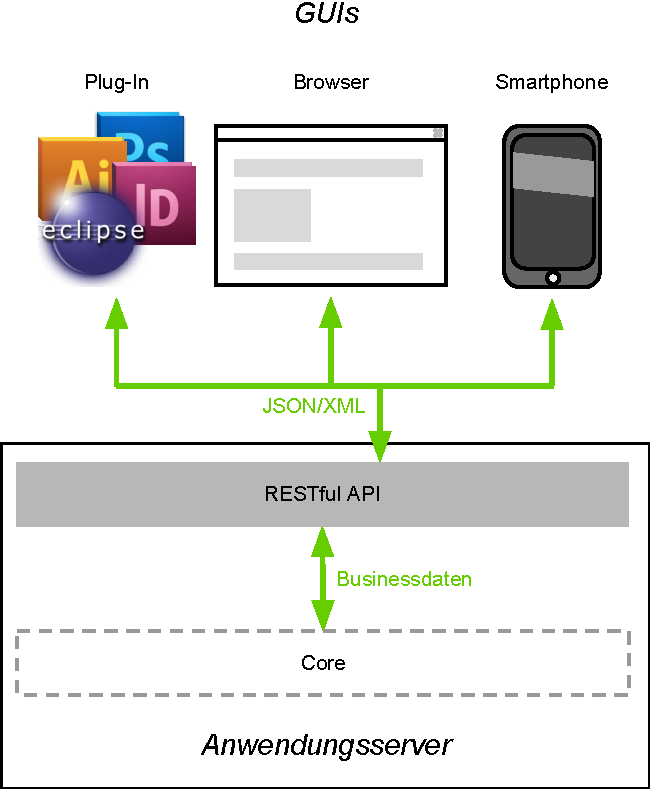
\includegraphics[width=0.65\textwidth]{media/ArtdesSystems.pdf}
\caption{Aufbau des System in stark vereinfachter Darstellung}
\label{chart:aufbaudessystems}
\end{center}
\end{figure}

\subsubsection{Browserbasierte Web-Anwendung} 

Diese Klasse von Anwendung verwendet einen Webbrowser als Laufzeitumgebung. Dabei stellt der Browser das GUI der Anwendung mit Hilfe von HTML, CSS und JavaScript dar, die Businesslogik und die Datenhaltung wird auf einem Server ausgeführt, mit der die GUI mithilfe einer Schnittstelle kommuniziert. Abbildung~\ref{chart:aufbaudessystems}~(S.\pageref{chart:aufbaudessystems}) zeigt den Aufbau des Systems in stark vereinfachter Darstellung. War es in den letzten Jahren noch üblich, dass Fragmente des GUIs mit serverseitigen Template-Sprachen erzeugt wurden (vgl.~\cite[S.48]{dunkel2008systemarchitekturen}) hat die zunehmende Verbreitung von mobilen Clients ein Umdenken zur Folge. Zum einen stellen Desktop-Clients, mobile Browser-Clients und native Apps zwar die gleichen Daten eines Systems dar, verwenden dafür aber nicht zwangsläufig die gleiche GUI-Technologie. Zum anderen werden Clients immer leistungsstärker, selbst Einsteiger-SmartPhones haben inzwischen CPUs mit mindestens dreistelligem Megahertz-Wert. Diese Entwicklung führt gerade bei Web-Anwendungen, auch Rich Internet Applications (RIAs) genannt, zu der Idee, Architekturen zu entwickeln, bei denen serverseitig keine GUI-Komponenten mehr erzeugt werden (vgl.~\cite{maccaw2011javascript}). Clients kommunizieren über Schnittstellen mit dem Server und tauschen nur noch reine Daten aus. Dies hat mehrere Vorteile. Zum einen muss serverseitig kein Modell der clientseitigen Darstellung verwaltet werden, zum anderen verkleinert sich die Menge der transferierten Daten zwischen Client und Server erheblich. Dies hat besonders bei Benutzern mit langsamen oder schlechten Datenverbindungen im Mobilfunk-Netz große Vorteile. Für Webanwendungen bedeutet dass diese das zur Darstellung benötigte HTML mit Hilfe von JavaScript selber direkt im Client erzeugen. Beim ersten Besuch einer Internetseite müssen lediglich einmal die JavaScript-Dateien und benötigte statische Ressourcen wie CSS-Dateien, Bilder und ein statischer HTML-Grundaufbau geladen werden. Anschließend werden nur noch die für die jeweilige Aktion benötigten Daten mit Hilfe von JavaScript zwischen der Anwendung und dem Server ausgetauscht. Mobile Endgeräte, die über eigene GUI-Toolkits verfügen, oder Software von Drittanbietern können dann die selben Schnittstellen verwenden, ohne dass serverseitige Anpassungen vorgenommen werden müssen. 

Web-Anwendung haben den Vorteil, dass sie ohne Installation auf dem Rechner des Benutzers lauffähig sind. Sie können als unmittelbar verwendet werden. Kompaitibilätsprobleme mit alten Browser-Versionen (z.B. dem \trademark{Internet Explorer 6}) können inzwischen mit Hilfe des \trademark{ChromeFrame}\footnote{\url{https://developers.google.com/chrome/chrome-frame/}} komfortable umgangen werden. Der Umfang an frei verfügbaren Bibliotheken zur Erstellung attraktiver und angenehm benutzbarer Anwendungen auf Basis von HTML ist riesig. Web-Anwendungen können mit wenig Aufwand auch auf mobilen Endgeräten eingesetzt werden, da Technologien zur platformabhängigen Anpassung der Darstellung (z.B. CSS-Mediaqueries) existierten. Insgesamt sind Webbrowser der aktuellen Generation mächtige Werkzeuge zur Erstellung von CRUD-Anwendungen. \cite{ms-key-software-development-trends} Die allgemeinen Vorteile einer browserbasierten Software, auch als \emph{Software as as Service} (SaaS) oder \emph{Application Service Provider} (ASP) Modell bekannt, liegen auf der Hand und werden an dieser Stelle nicht detailliert ausgeführt. Um nur einen zu nennen: die Möglichkeit, die Software jederzeit und für alle Mitarbeiter gleichzeitg ohne deren Zutun aktualisieren zu können, eliminiert vielfältige Probleme, die sonst in Umgebungen entstehen, in denen unterschiedliche Programmversionen existieren.

\subsubsection{Schnittstellen} 

Die Verwenden einer einheitlichen Schnittstelle durch alle Clients ermöglicht ein konsistentes Verhalten der Anwendungen über alle Zugangswege hinweg und ist besonders in Fall dieser Anwendung von Bedeutung, da die Benutzer des Systems wünschen, dass sich die Texte direkt innerhalb ihrer bevorzugten Werkzeuge abrufen und einbinden lassen. Dies ist nur mit Hilfe von Plugin-Ins möglich, die in der jeweiligen Umgebung der Software entwickelt werden müssen. Aus diesem Grund ist es ungvermeidlich, dass für alle Funktionen des Systems eine öffentliche Schnittstelle existiert.

Als Protokoll zur Kommunikation zwischen Clients und Server hat sich REST bewährt. Die Struktur des Protokolls ist direkt mit dem HTTP-Protokoll vebunden, so ist die Verarbeitung von REST-Anfragen serverseitig leicht mit Web-Frameworks zu implementieren, da diese von sich aus bereits für diese Art von Anfragen ausgelegt sind. Clientseitig wird lediglich ein HTTP-Client benötigt sowie Module zum Parsen von JSON- oder XML-Datenstrukturen -- Voraussetzungen, die von Browsern und SmartPhones erfüllt werden. JSON hat im Vergleich zu SOAP den Vorteil, dass es nicht versucht die Architektur der zugrundeliegenden Software nach außen abzubilden, so muss sich der Client nicht an bestimmte Reihenfolgen im Aufruf von Methoden halten. In der REST-Welt sind alle Operationen atomar und können ohne Vorbedingung gestellt werden. In der Praxis ist dies nicht immer umsetzbar, REST fordert serverseitig Zustandslosigkeit, die aber bei Systemen in denen Daten gespeichert und verändert werden nicht realisierbar ist. Aufgrund seines flexibleren Aufbaus, der Möglichkeit ausgewählte Anfragen leicht mit HTTP-Caches zu beschleunigen und der freien Wahl der Nachrichtenformats ist REST aus Sicht des Autors die besser Wahl zur Implementierung der Schnittstellenkommunikation.

\subsubsection{Zugang}

Diese Konzept macht es möglich, jedem Mitarbeiter den passenden Zugang zu ermöglichen, im Einzelnen sind das:

\paragraph{Browserbasierter Zugang vom Desktop} Den Webbrowser werden alle Mitarbeiter verwenden, da in diesem GUI alle Funktionen der Anwendung implementiert sind.

\paragraph{Browserbasierter Zugang von SmartPhones} Auf gängigen SmartPhones sind Browser vorhanden, die in der Lage sind, die selben Inhalten anzuzeigen, wie ihr Desktop-Equivalent. Aufgrund der deutlich kleineren Bildschirmgröße und dem fehlen einer Maus ist es aber sinnvoll, dem Rechnung zu tragen und eine angepasste Version der Anwendung für diese Geräte bereit zustellen. 

\paragraph{Zugang direkt über die Schnittstellen} Vor allem im Bereich der Software-Entwicklung wird der direkte Zugriff der Entwickler auf die Schnittstellen der Anwendung eine wichtige Rolle spielen. So können diese die Integration des Systems in ihren Entwicklungsprozess optimal an die jeweiligen Bedürfnisse anpassen.

\paragraph{Exporte} Die Möglichlichkeit, die Texte des Projektes in verschiedene Formate zu exportieren ist eine wichtige Funktion. Sie ermöglicht zum einen die Übernahme in System und Programme, deren Anbindung nicht möglich oder gewünscht ist und schafft zum anderen die Möglichkeit, ähnlich wie Schnittstellen, die verarbeiteten Daten auf eine Art und Weise zu verwenden, die nicht vorhergesehen wurde oder nicht im Sinne der Anwendung liegt.

\paragraph{Zugang über Plug-Ins} Besonders für Mitarbeiter in der Produktion kann es wichtig sein, auf ihre angestammten Werkzeuge nicht verzichten zu müssen. Plug-Ins, also Erweiterungen für diese Werkzeuge, integrieren dann Teile der Funktionen der Anwendung in diese Werkzeuge. Beispielsweise könnte es ein Plug-In für \trademark{Adobe InDesign} ermöglichen, auf die Texte aus dem System zuzugreifen und diese direkt in Text-Rahmen im \trademark{InDesign}-Dokument zu übernehmen, so dass Copy\&Paste der Texte aus der Webanwendung oder einem exportierten Dokument entfallen kann.

\paragraph{Benachrichtigungen} Benachrichtigungen sind eine Form des Zugangs, die es Benutzern des Systems ermöglicht, über bestimmte Ereignisse informiert zu werden. Benachrichtigungen können in Form von E-Mails, SMS, über soziale Netzwerke wie Twitter, über Chat-Dienste wie Skype, IRC statt finden. Hierbei werden Information zu einem Ereignis übertragen z.B. der Status-Änderungen eines Textes. Denkbar sind auch auch Push-Exporte der Texte aufgrund eines bestimmten Ereignisses, z.B. der FTP-Export der Texte als CSV-Datei, sobald das Projekt abgschlossen ist oder Änderungen freigegeben wurden.

\paragraph{Software von Drittanbietern} Dadurch, dass alle Funktionen der Anwendung über eine Api exponiert werden, sind auch fremde Softwarehersteller in der Lage, Teile der Funktionen oder die gesamte Anwendung in einer eigenen GUI zu implementieren. So können Bedürfnisse von Anwendergruppen mit besonderen Anforderungen abgedeckt werden, die bei der Konzipierung der Anwendung nicht berücksichtigt wurden.

\subsubsection{Überblick}

Abbildung~\ref{chart:gesamtessystem}~(S.\pageref{chart:gesamtessystem}) liefert einen Überblick über den Aufbau des gesamten Systems:

\begin{figure}[htb]
\begin{center}
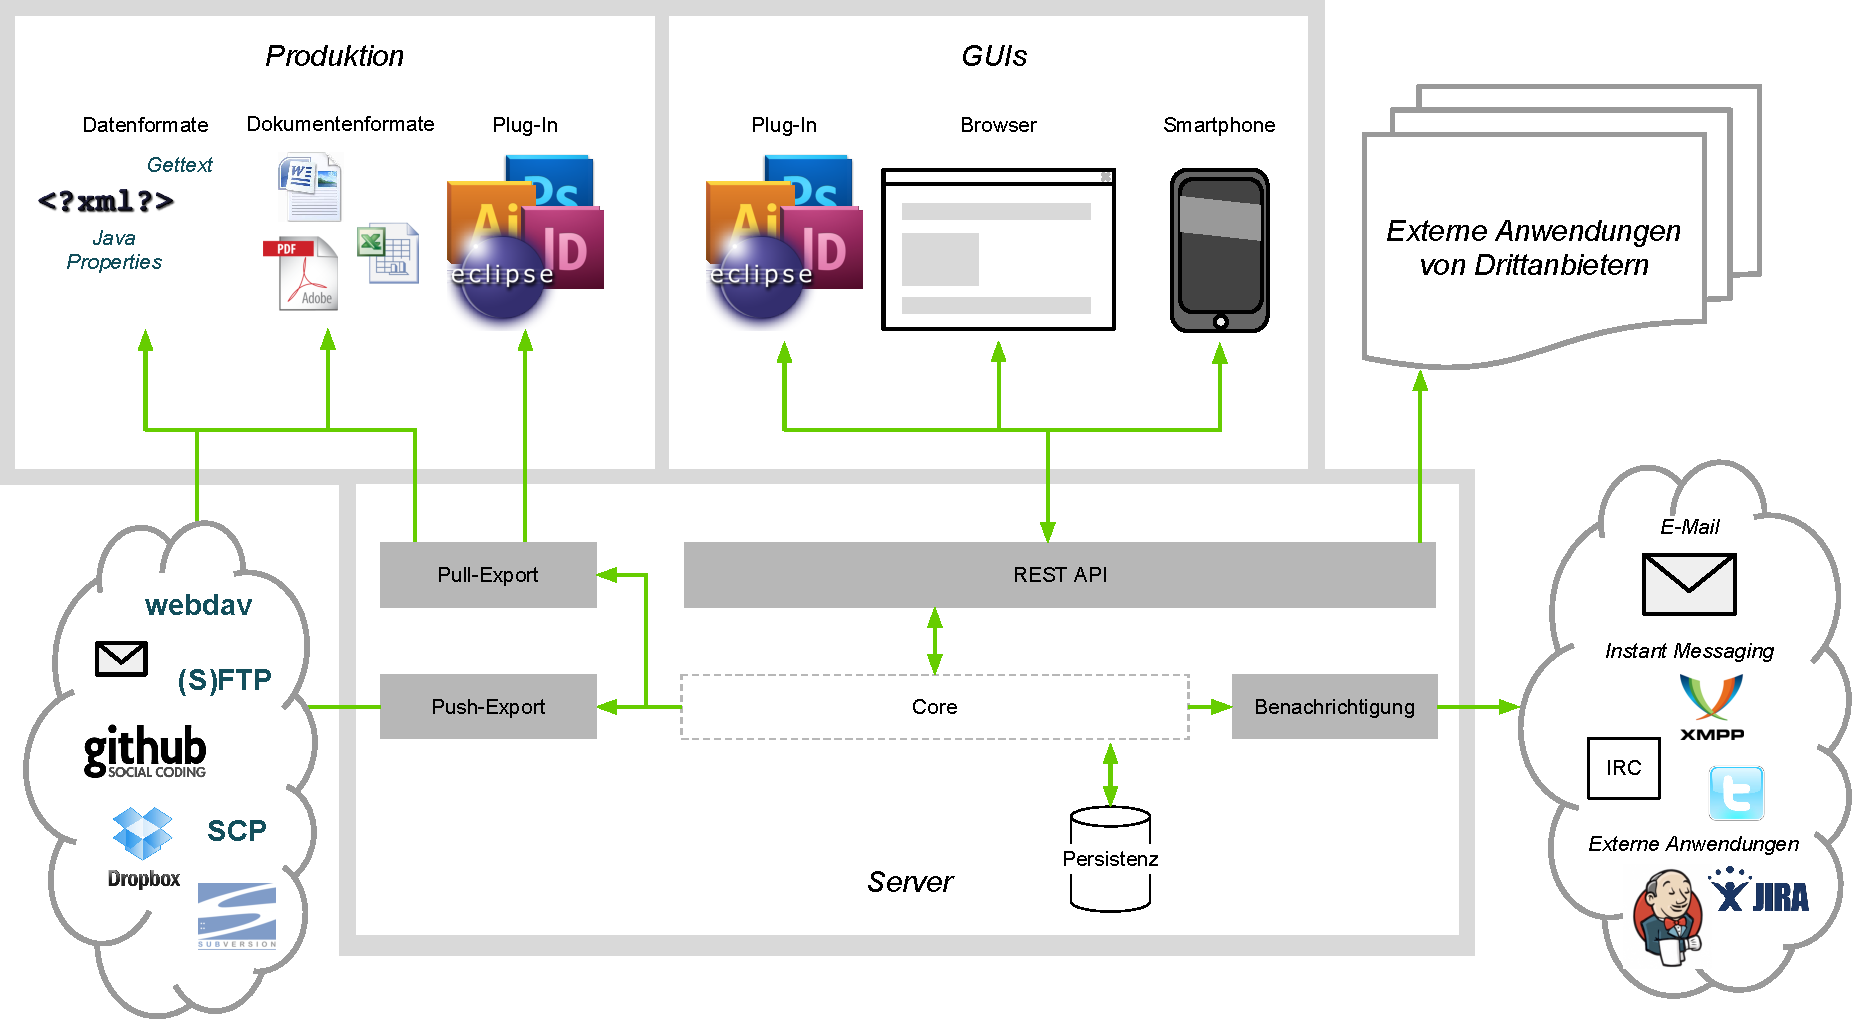
\includegraphics[width=\textwidth]{media/GesamtesSystem.pdf}
\caption{Aufbau des gesamten Systems im Überblick}
\label{chart:gesamtessystem}
\end{center}
\end{figure}

Die Zentrale Komponente der Anwendung bildet der Server. Für die Benutzer erfolgt der Zugriff mit Hilfe einer GUI, die mit der REST-API des Servers kommuniziert. Eine browserbasierte GUI auf Basis von HTML5 und JavaScript bildet den Hauptzugang zum System, der auch auf SmartPhones verwendet werden kann. Zusätzlich gibt es spezielle Plugins für Adobe-Produkte und weitere wichtige Produktionsumgebungen. Auch native GUIs für Smartphones verwenden die gleiche API. Die Schnittstellen können auch von Drittanbietern dazu verwendet werden, eigenen Clients für das System zu entwickeln. In die Endprodukte gelangen die Texten über den Export, exportiert wird dabei in viele Formate, neben Datenformaten wie z.B. XML werden auch Dokumentenformate wie z.B. Word exportiert. Der Export kann durch den Anwender erzeugt werden (\emph{Pull-Export}), aber auch automatisch, z.B. nach festgelegten Zeitplänen oder Ereignissen erfolgen. Dieser \emph{Push-Export} erfolgt auf je nach Projekt festlegbaren Orte, wie z.B. FTP-Server oder Versionsverwaltungssysteme. Die Benachrichtigungen über Aufgaben und Änderungen an Texten kann via E-Mail, aber auch mittels Instant-Messaging-Systeme oder durch den Aufruf fremde API-Endpunkte erfolgen.